\chapter{\texorpdfstring{\Glsentrytext{fpga}}{FPGA} Implementation}\label{chap:FPGA_Implementation}

\section{About}\label{sec:About}
\paragraph{}The Chipyard Framework contains initial support for FPGA development and simulation of SoC designs. 
At the moment this support is very limited, and is in active development. 
As of \today, the best support for FPGA Development for the Arty 35T FPGA comes from a branch of Chipyard called "arty-spi-flash". 
This branch fixes the UART implementation, and enables the SPI Flash storage on the Arty FPGA to allow users to store programs on the FPGA


\section{Prerequisites}\label{sec:Prerequisites}
To assist with the proper setup, we approached the FPGA implementation of an SoC by following the "SiFive Freedom E310 Arty FPGA Dev Kit Getting Started Guide".~\cite{FreedomDevGuide}
This outlined many of the steps we would eventually need to take, starting with purchasing an \href{https://www.digikey.com/en/products/detail/olimex-ltd/ARM-USB-TINY-H/3471388}{Olimex JTAG Debugger}~\cite{OlimexJTAG}. 
Once the final image is flashed to the FPGA, the debugger will allow the user to upload C programs and execute them on the RISC-V processor. 

\begin{figure}[h]
	\centering
	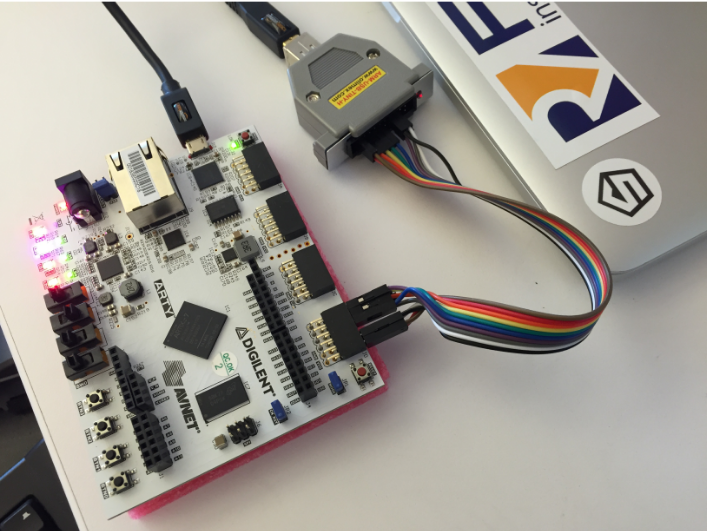
\includegraphics[width=0.7\linewidth]{Images/OlimexSetup}
	\caption[]{Olimex Debugger Setup}
	\label{fig:olimexsetup}
	\cite[p.~5]{FreedomDevGuide}
\end{figure}



%%% Local Variables:
%%% mode: latex
%%% TeX-master: "../doc"
%%% End:
